\documentclass[11pt]{article}
\usepackage[utf8]{inputenc}
\usepackage[margin=1in]{geometry}
\usepackage{booktabs}
\usepackage{graphicx}
\usepackage{amsmath}
\usepackage{url}
\usepackage[hidelinks]{hyperref}
\graphicspath{{../results/figures/}}

\title{Token-Accounting Integrity: Systematizing and Evaluating\\
Client-Side Metering Evasion in LLM-Powered Applications}
\author{(anonymized for review)}
\date{}

\begin{document}
\maketitle

\begin{abstract}
LLM applications bill by metering token and inference consumption. Existing security
work on LLM billing runs in two directions: a dishonest \emph{provider} over-charging an
honest client (CoIn; Invisible Tokens, Visible Bills; Token Inflation), and a third
party inflating a \emph{victim}'s bill (Denial-of-Wallet; LLMjacking). The inverse---a
legitimate but dishonest \emph{client} exploiting LLM-billing-specific weaknesses to
under-pay---has no taxonomy, benchmark, or measured defense evaluation. We do not claim
new attack primitives; the enabling mechanisms already exist as scattered
deployed-gateway bugs, generic weaknesses, and payment folklore. Instead we
\emph{systematize} client-side metering evasion around a single safety invariant---%
\emph{no served inference without a committed, non-refunded, server-authoritative
debit}---and \emph{measure} it on a reproducible, vulnerable-by-construction testbed
(FastAPI + PostgreSQL + Redis + a deterministic mock model, no GPU). We operationalize
two LLM-relevant accounting dimensions---metering-commit timing (M1) and usage-record
authority (M2)---across representative architectures, using a generic credit-decrement
race (B0) as a known baseline. We quantify leakage, attack-success rate, detectability,
and defense overhead, with per-request-ledger integrity gates. Aborting a stream just
before a post-hoc commit yields up to the full request cost for free (invariant
violated at abort points before completion; zero after); a client-authoritative usage
record leaks up to 58--74\% of the true inference value depending on the billing basis;
and in every case a server-authoritative defense reduces leakage to zero at modest
cost. All figures regenerate from raw data.
\end{abstract}

\section{Introduction}
Usage-based billing has become the default commercial model for LLM APIs and agents.
Because the billed unit---the token---is produced by opaque, streamed, non-deterministic
inference, the \emph{accounting} pipeline (authorize, meter, commit a charge) is itself
security-sensitive. Recent work studies dishonest \emph{providers} inflating that
accounting against honest users, and availability attacks that drain a victim's budget.
We study the missing quadrant: an honest provider and a \emph{dishonest client} that
seeks metered inference while under-paying (Table~\ref{tab:quadrant}).

We are deliberately adversarial about our own novelty. The underlying mechanisms are
\emph{known}: a deployed LLM gateway already refunds pre-consumed quota when a final
usage block is missing after disconnect (new-api \#5235); ``never trust client input''
is CWE-807 and is already mitigated against encoding-induced ``silent zero-debit'' in a
metered-token proxy (aperture \#247); and concurrent quota-decrement races are a classic
web-race primitive with a recent CVE (Tyk CVE-2026-31873). Our contribution is not to
discover these but to (i) place them in a taxonomy unified by one safety invariant,
(ii) build a reproducible testbed and \emph{measure} their economic leakage, attack
success, and detectability across architectures, and (iii) evaluate server-side defenses
and their overhead.

\begin{table}[t]\centering
\caption{Directions of LLM-billing security. This paper targets the shaded cell.}
\label{tab:quadrant}
\begin{tabular}{lll}
\toprule
 & Inflate cost & Evade cost \\
\midrule
Provider dishonest & CoIn / Invisible Tokens (covered) & --- \\
Client dishonest & Denial-of-Wallet / LLMjacking (covered) & \textbf{this paper} \\
\bottomrule
\end{tabular}
\end{table}

\paragraph{Research questions.}
\textbf{RQ1} How does the placement of metering authority and financial commitment
affect client-side under-payment? \textbf{RQ2} How much inference value can a dishonest
client obtain without authoritative billing, across architectures? \textbf{RQ3} Which
failures are visible to the application's own logs/reconciliation? \textbf{RQ4} Which
server-side defenses eliminate the violation, and at what cost?

\section{Threat Model}
Honest provider; dishonest client with valid credentials. The client fully controls its
own requests: timing, concurrency, connection lifetime (it may abort at any moment), and
any client-declared fields (e.g.\ a \texttt{usage} object). It cannot read/write other
tenants' state, forge the provider's own upstream usage metadata, or break
authentication (that would be LLMjacking). Success on request $r$: it receives inference
value $C(r)$ but the account is net-charged less. All attacks run only against the local
testbed; no third-party system is touched.

\section{Formal Model}
For request $r$ let $S(r)\in\{0,1\}$ be served, $C(r)$ the authoritative cost of the
inference obtained, and $\mathrm{NetDebit}(r)=\text{committed}(r)-\text{refund}(r)$.
Under-payment is
\[
\mathrm{Leak}(r)=S(r)\,C(r)-\mathrm{NetDebit}(r),\qquad
\text{efficiency}=\frac{\max(\mathrm{Leak}(r),0)}{C(r)} .
\]
The safety invariant is $S(r)=1 \Rightarrow \mathrm{NetDebit}(r)\ge C(r)$, and the
system must satisfy accounting conservation
$\sum_r \mathrm{NetDebit}(r) = B_\text{init}-B_\text{final}$, which we assert on every
trial as an integrity gate.

\section{Taxonomy}
All mechanisms violate the one invariant and differ in \emph{where} the integrity
boundary sits in \emph{authorize $\to$ [commit timing] $\to$ inference $\to$ [usage
authority] $\to$ [atomic decrement] $\to$ debit}.

\paragraph{M1 --- Metering-commit timing.} When is the charge irrevocable relative to
streamed delivery? Architectures: \texttt{pre\_debit} (safe), \texttt{reserve\_reconcile}
(safe, recommended), \texttt{post\_completion} (leaks: no debit on abort),
\texttt{reserve\_refund\_on\_abort} (leaks: refunds the whole reserve on a missing final
usage block---the new-api \#5235 pattern).

\paragraph{M2 --- Usage-record authority.} Who sets the billed quantity? Architectures
span client-authoritative to server-authoritative: \texttt{client},
\texttt{client\_logged}, \texttt{client\_total} (all leak), and \texttt{upstream},
\texttt{server\_recount}, \texttt{hybrid\_reconcile} (safe), yielding a detection
spectrum D0--D3.

\paragraph{B0 --- Credit/quota-decrement race (baseline, known).} Non-atomic
check-then-decrement TOCTOU; concurrency multiplies the allowance (Kettle;
CVE-2026-31873). It answers the LLM-specificity control (Gate~C): B0 works unchanged
against any non-LLM API; M1/M2 depend on streaming inference and token-usage semantics
respectively.

\paragraph{Killed.} M3 (inference-cache billing) was killed at its decision gate---it
reduces to solved idempotency, generic cache authorization, and a billing-policy choice.
Old classes 4 (quota race $\to$ B0) and 5 (entitlement tampering $\to$ OWASP API1/API3)
were killed in the Phase~1 audit.

\section{Testbed and Methodology}
FastAPI/uvicorn gateway, PostgreSQL~16 (\texttt{READ COMMITTED}), Redis~7, deterministic
mock LLM streaming tokens as a pure function of (prompt, seed); Docker Compose on one
commodity host. B0 tables are frozen from the validated baseline; M1/M2 use separate
tables so the baseline cannot regress. Category-wise exact-\texttt{Decimal} pricing over
\{input, output, cached, reasoning\} in three tiers (low/medium/high); leakage efficiency
is tier-invariant. Sweeps: B0 concurrency $\{1,2,5,10,20,30,50\}\times30$; M1
architecture$\times$abort\%$\{0..100\}\times$tier$\times10$ (840 records) via real SSE
streams the client aborts; M2 architecture$\times$manipulation$\times$tier$\times10$
(1440 records). Sample sizes are justified from measured dispersion: leak magnitude is
deterministic (std $=0$), so proportion (Wilson) intervals bound precision. Every figure
is re-derived from the per-request ledger and cross-checked against the stored value; all
trials reconcile.

\section{Results}
Integrity: independent re-derivation passes with 0 problems over 420 B0 trials, 840 M1
records, and 1440 M2 records; all trials reconcile; controls pass 19/19 (B0) and 16/16
(M1/M2).

\paragraph{B0 (Table~\ref{tab:b0}).} Vulnerable leaks for concurrency $\ge2$ (never at
1); trial-ASR $=1.0$; the hardened atomic decrement leaks \$0 at all concurrency.

\paragraph{M1 (Fig.~\ref{fig:m1}, Table~\ref{tab:m1}).} The vulnerable architectures
have request-ASR $1.00$ and invariant-violation $1.00$ at every abort point before
completion; leak rises monotonically with delivered tokens (mean \$0.054 at 50\%,
\$0.096 at 90\%, medium tier) and collapses to \$0 at completion. Safe architectures leak
\$0 everywhere. ``Debit after completion'' and ``refund the reserve on abort'' are the
same failure.

\paragraph{M2 (Fig.~\ref{fig:m2}, Table~\ref{tab:m2}).} Client-authoritative billing
leaks; leakage efficiency reaches $0.58$ for a 90\% output under-report and $0.74$ for a
total/subtotal mismatch under flat total pricing. Crucially, the \emph{exploitable
manipulation set depends on the billing basis} (category vs total). Every
server-authoritative architecture drives leakage efficiency to $0.00$ across all eight
manipulations (detection D3).

\paragraph{Defense overhead (RQ4).} \texttt{reserve\_reconcile} adds $+9.8$\,ms mean over
\texttt{post\_completion} (two extra atomic writes); \texttt{server\_recount} adds
$+0.1$\,ms over \texttt{client} in the testbed---with the caveat that the mock makes the
recount nearly free (a production tokenizer pass is the real, unmeasured cost).

\begin{table}[t]
\centering
\small
\caption{B0 baseline: credit-decrement race (30 reps/cell).}
\label{tab:b0}
\resizebox{\linewidth}{!}{%
\begin{tabular}{lrrrrrr}
\toprule
posture & conc & served & \$-leak & trial ASR & req ASR & detect \\
\midrule
hardened & 1 & 1.0 & 0.0000 & 0.00 & 0.000 & none \\
hardened & 2 & 2.0 & 0.0000 & 0.00 & 0.000 & none \\
hardened & 5 & 5.0 & 0.0000 & 0.00 & 0.000 & none \\
hardened & 10 & 10.0 & 0.0000 & 0.00 & 0.000 & none \\
hardened & 20 & 10.0 & 0.0000 & 0.00 & 0.000 & none \\
hardened & 30 & 10.0 & 0.0000 & 0.00 & 0.000 & none \\
hardened & 50 & 10.0 & 0.0000 & 0.00 & 0.000 & none \\
vulnerable & 1 & 1.0 & 0.0000 & 0.00 & 0.000 & none \\
vulnerable & 2 & 2.0 & 0.0990 & 1.00 & 0.500 & partial \\
vulnerable & 5 & 5.0 & 0.3960 & 1.00 & 0.800 & partial \\
vulnerable & 10 & 10.0 & 0.8910 & 1.00 & 0.900 & partial \\
vulnerable & 20 & 20.0 & 1.8810 & 1.00 & 0.950 & partial \\
vulnerable & 30 & 30.0 & 2.8710 & 1.00 & 0.967 & partial \\
vulnerable & 50 & 50.0 & 4.8510 & 1.00 & 0.980 & partial \\
\bottomrule
\end{tabular}
}
\end{table}

\begin{table}[t]
\centering
\caption{M1 metering-commit timing: leak vs. abort (medium tier, 10 reps).}
\label{tab:m1}
\begin{tabular}{lrrrrrr}
\toprule
architecture & abort\% & delivered & mean leak & req ASR & inv.viol & detect \\
\midrule
pre\_debit & 0 & 1 & 0.0000 & 0.00 & 0.00 & n/a \\
pre\_debit & 10 & 7 & 0.0000 & 0.00 & 0.00 & n/a \\
pre\_debit & 25 & 17 & 0.0000 & 0.00 & 0.00 & n/a \\
pre\_debit & 50 & 34 & 0.0000 & 0.00 & 0.00 & n/a \\
pre\_debit & 75 & 52 & 0.0000 & 0.00 & 0.00 & n/a \\
pre\_debit & 90 & 62 & 0.0000 & 0.00 & 0.00 & n/a \\
pre\_debit & 100 & 69 & 0.0000 & 0.00 & 0.00 & n/a \\
reserve\_reconcile & 0 & 1 & 0.0000 & 0.00 & 0.00 & n/a \\
reserve\_reconcile & 10 & 7 & 0.0000 & 0.00 & 0.00 & n/a \\
reserve\_reconcile & 25 & 17 & 0.0000 & 0.00 & 0.00 & n/a \\
reserve\_reconcile & 50 & 34 & 0.0000 & 0.00 & 0.00 & n/a \\
reserve\_reconcile & 75 & 52 & 0.0000 & 0.00 & 0.00 & n/a \\
reserve\_reconcile & 90 & 62 & 0.0000 & 0.00 & 0.00 & n/a \\
reserve\_reconcile & 100 & 69 & 0.0000 & 0.00 & 0.00 & n/a \\
post\_completion & 0 & 1 & 0.0045 & 1.00 & 1.00 & D0 \\
post\_completion & 10 & 7 & 0.0135 & 1.00 & 1.00 & D0 \\
post\_completion & 25 & 17 & 0.0285 & 1.00 & 1.00 & D0 \\
post\_completion & 50 & 34 & 0.0540 & 1.00 & 1.00 & D0 \\
post\_completion & 75 & 52 & 0.0810 & 1.00 & 1.00 & D0 \\
post\_completion & 90 & 62 & 0.0960 & 1.00 & 1.00 & D0 \\
post\_completion & 100 & 69 & 0.0000 & 0.00 & 0.00 & n/a \\
reserve\_refund\_on\_abort & 0 & 1 & 0.0045 & 1.00 & 1.00 & D0 \\
reserve\_refund\_on\_abort & 10 & 7 & 0.0135 & 1.00 & 1.00 & D0 \\
reserve\_refund\_on\_abort & 25 & 17 & 0.0285 & 1.00 & 1.00 & D0 \\
reserve\_refund\_on\_abort & 50 & 34 & 0.0540 & 1.00 & 1.00 & D0 \\
reserve\_refund\_on\_abort & 75 & 52 & 0.0810 & 1.00 & 1.00 & D0 \\
reserve\_refund\_on\_abort & 90 & 62 & 0.0960 & 1.00 & 1.00 & D0 \\
reserve\_refund\_on\_abort & 100 & 69 & 0.0000 & 0.00 & 0.00 & n/a \\
\bottomrule
\end{tabular}
\end{table}

\begin{table}[t]
\centering
\caption{M2 usage-record authority: leakage efficiency by manipulation (medium tier, concurrency=1).}
\label{tab:m2}
\begin{tabular}{lrrrrr}
\toprule
architecture & manipulation & leak eff. & req ASR & inv.viol & detect \\
\midrule
client & honest & 0.00 & 0.00 & 0.00 & n/a \\
client & under\_report\_output\_50 & 0.32 & 1.00 & 1.00 & D0 \\
client & under\_report\_output\_90 & 0.58 & 1.00 & 1.00 & D0 \\
client & under\_report\_input\_50 & 0.01 & 1.00 & 1.00 & D0 \\
client & drop\_reasoning & 0.32 & 1.00 & 1.00 & D0 \\
client & inflate\_cached & 0.31 & 1.00 & 1.00 & D0 \\
client & total\_mismatch & 0.00 & 0.00 & 0.00 & n/a \\
client & rounding\_shave & 0.04 & 1.00 & 1.00 & D0 \\
client\_logged & honest & 0.00 & 0.00 & 0.00 & n/a \\
client\_logged & under\_report\_output\_50 & 0.32 & 1.00 & 1.00 & D1 \\
client\_logged & under\_report\_output\_90 & 0.58 & 1.00 & 1.00 & D1 \\
client\_logged & under\_report\_input\_50 & 0.01 & 1.00 & 1.00 & D1 \\
client\_logged & drop\_reasoning & 0.32 & 1.00 & 1.00 & D1 \\
client\_logged & inflate\_cached & 0.31 & 1.00 & 1.00 & D1 \\
client\_logged & total\_mismatch & 0.00 & 0.00 & 0.00 & n/a \\
client\_logged & rounding\_shave & 0.04 & 1.00 & 1.00 & D1 \\
client\_total & honest & 0.00 & 0.00 & 0.00 & n/a \\
client\_total & under\_report\_output\_50 & 0.27 & 1.00 & 1.00 & D0 \\
client\_total & under\_report\_output\_90 & 0.53 & 1.00 & 1.00 & D0 \\
client\_total & under\_report\_input\_50 & 0.00 & 0.00 & 0.00 & n/a \\
client\_total & drop\_reasoning & 0.27 & 1.00 & 1.00 & D0 \\
client\_total & inflate\_cached & 0.00 & 0.00 & 0.00 & n/a \\
client\_total & total\_mismatch & 0.74 & 1.00 & 1.00 & D0 \\
client\_total & rounding\_shave & 0.00 & 0.00 & 0.00 & n/a \\
upstream & honest & 0.00 & 0.00 & 0.00 & n/a \\
upstream & under\_report\_output\_50 & 0.00 & 0.00 & 0.00 & n/a \\
upstream & under\_report\_output\_90 & 0.00 & 0.00 & 0.00 & n/a \\
upstream & under\_report\_input\_50 & 0.00 & 0.00 & 0.00 & n/a \\
upstream & drop\_reasoning & 0.00 & 0.00 & 0.00 & n/a \\
upstream & inflate\_cached & 0.00 & 0.00 & 0.00 & n/a \\
upstream & total\_mismatch & 0.00 & 0.00 & 0.00 & n/a \\
upstream & rounding\_shave & 0.00 & 0.00 & 0.00 & n/a \\
server\_recount & honest & 0.00 & 0.00 & 0.00 & n/a \\
server\_recount & under\_report\_output\_50 & 0.00 & 0.00 & 0.00 & n/a \\
server\_recount & under\_report\_output\_90 & 0.00 & 0.00 & 0.00 & n/a \\
server\_recount & under\_report\_input\_50 & 0.00 & 0.00 & 0.00 & n/a \\
server\_recount & drop\_reasoning & 0.00 & 0.00 & 0.00 & n/a \\
server\_recount & inflate\_cached & 0.00 & 0.00 & 0.00 & n/a \\
server\_recount & total\_mismatch & 0.00 & 0.00 & 0.00 & n/a \\
server\_recount & rounding\_shave & 0.00 & 0.00 & 0.00 & n/a \\
hybrid\_reconcile & honest & 0.00 & 0.00 & 0.00 & n/a \\
hybrid\_reconcile & under\_report\_output\_50 & 0.00 & 0.00 & 0.00 & n/a \\
hybrid\_reconcile & under\_report\_output\_90 & 0.00 & 0.00 & 0.00 & n/a \\
hybrid\_reconcile & under\_report\_input\_50 & 0.00 & 0.00 & 0.00 & n/a \\
hybrid\_reconcile & drop\_reasoning & 0.00 & 0.00 & 0.00 & n/a \\
hybrid\_reconcile & inflate\_cached & 0.00 & 0.00 & 0.00 & n/a \\
hybrid\_reconcile & total\_mismatch & 0.00 & 0.00 & 0.00 & n/a \\
hybrid\_reconcile & rounding\_shave & 0.00 & 0.00 & 0.00 & n/a \\
\bottomrule
\end{tabular}
\end{table}

\begin{table}[t]
\centering
\small
\caption{Architecture safety summary across all attacks and tiers.}
\label{tab:defense}
\begin{tabular}{lrrrr}
\toprule
mech & architecture & verdict & max req ASR & best detect \\
\midrule
M1 & pre\_debit & safe & 0.00 & D3 \\
M1 & reserve\_reconcile & safe & 0.00 & D3 \\
M1 & post\_completion & LEAKS & 1.00 & D0 \\
M1 & reserve\_refund\_on\_abort & LEAKS & 1.00 & D0 \\
M2 & client & LEAKS & 1.00 & D0 \\
M2 & client\_logged & LEAKS & 1.00 & D1 \\
M2 & client\_total & LEAKS & 1.00 & D0 \\
M2 & upstream & safe & 0.00 & D3 \\
M2 & server\_recount & safe & 0.00 & D3 \\
M2 & hybrid\_reconcile & safe & 0.00 & D3 \\
\bottomrule
\end{tabular}
\end{table}


\begin{figure}[t]\centering
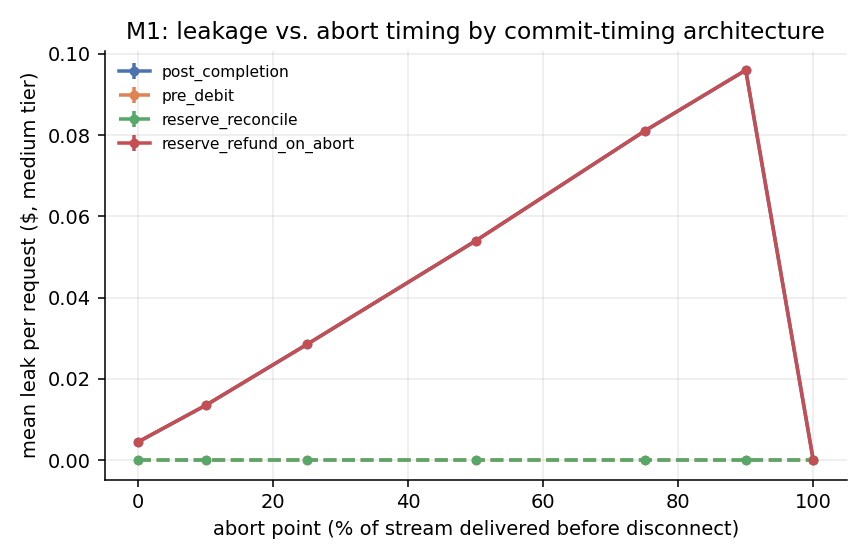
\includegraphics[width=0.72\linewidth]{fig_m1_abort_curve.png}
\caption{M1: leakage vs.\ abort timing. Vulnerable architectures peak just before the
commit and collapse to \$0 at completion; safe architectures stay at \$0.}
\label{fig:m1}
\end{figure}

\begin{figure}[t]\centering
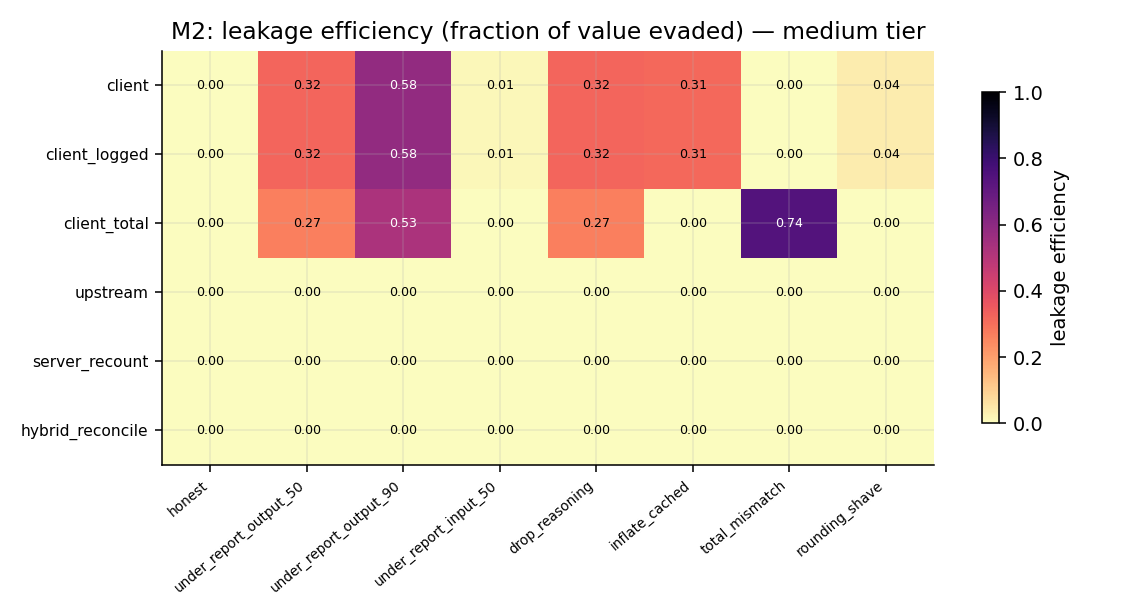
\includegraphics[width=0.92\linewidth]{fig_m2_efficiency_heatmap.png}
\caption{M2: leakage efficiency (fraction of value evaded) by architecture $\times$
manipulation (medium tier). Server-authoritative rows are all zero.}
\label{fig:m2}
\end{figure}

\begin{figure}[t]\centering
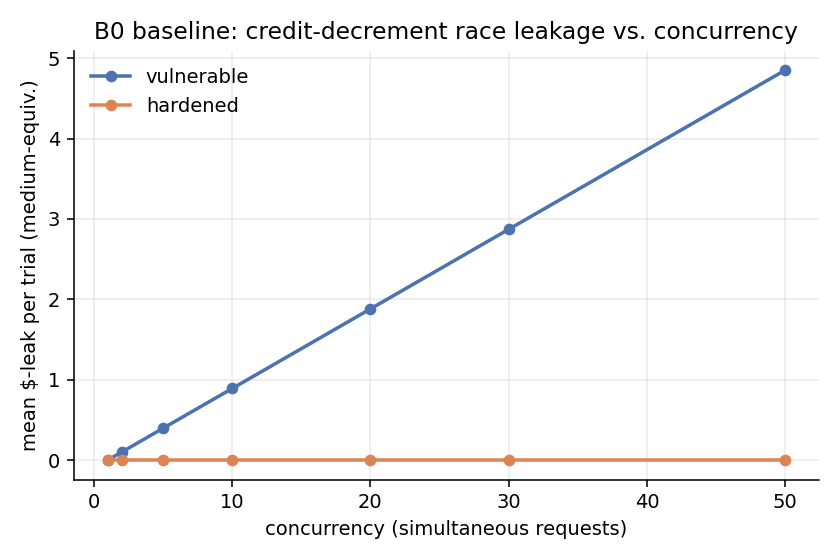
\includegraphics[width=0.6\linewidth]{fig_b0_concurrency.png}
\caption{B0 baseline: credit-decrement race leakage vs.\ concurrency.}
\label{fig:b0}
\end{figure}

\section{Defense Evaluation}
Each vulnerable architecture is paired with a server-side primitive: atomic
compare-and-decrement (B0), reserve-then-reconcile in a cancellation-shielded settlement
(M1), and server-authoritative recount (M2). Under every defense the invariant-violation
rate and leakage efficiency are zero across the full attack catalogue. Detection is a
second axis: logging a recount moves M2 from D0 (invisible) to D1 (reconcilable), and
request-time reconciliation reaches D3---a cheap, deployable intermediate step for
operators who cannot yet re-architect billing.

\section{Discussion, Threats to Validity, Disclosure}
The mechanisms are type-B reframes, not new primitives; the contribution is
systematization + measurement + defense, and we use bounded novelty language throughout.
Principal threats: the mock model makes the M2 recount defense nearly free (production
tokenizer cost unmeasured); single-node PostgreSQL and HTTP/1.1; M1/M2 are not evaluated
under concurrency (B0's axis). The ``no prior systematic study'' claim is a bounded
negative from targeted search, not a proof of non-existence. No third-party system was
tested; cited artifacts (new-api \#5235, aperture \#247, CVE-2026-31873) were already
public.

\section{Conclusion}
Client-side metering evasion in LLM applications is a coherent, measurable problem in the
one billing quadrant prior work leaves open. Two LLM-relevant dimensions---when billing
commits and who authoritatively counts usage---plus a generic race baseline, all reduce
to a single safety invariant, and all are closed by moving the authoritative,
irrevocable accounting event server-side. We release the testbed, harness, defenses, and
data so operators can measure their own gateways.

\end{document}
